\chapter{Results}
\label{resultS}
This chapter follows up the event selection and particle identification. All the conditions and cuts implemented in \autoref{analysis} helped sort through the massive number of events and pick the best candidates for further study. The focus of this chapter is on 2 particles: $K^0_S$ and $\Lambda^0$. Their peaks will be fitted with different distribution functions and results will be discussed. Part of search for $\Lambda^0$ are results for it's antiparticle $\overline{\Lambda}^0$. Differences between their production will be discussed. At the end of each section, exclusive production will be discussed. The analysis is still in progress and the results presented in this work have not yet been approved by the STAR collaboration for public presentation.
\section{Results for $K^0_S$}
\label{K0s}
Particle $K^0_S$ is one of two different neutral kaons, the other being $K^0_L$. The only difference between the two of them is their lifetime. The PDG value for lifetime of $K^0_S$ is $\tau_S = (8.954 \pm 0.004)10^{-11}$ s and for $K^0_L$ $\tau_L = (5.116 \pm 0.021)10^{-8}$ s. Kaons have spin 0 and parity -1. The dominant decay for $K^0_S$ is $\pi^+ \pi^-$. The other major decay is $\pi^0 \pi^0$. There are other, exotic decay channels, but their incidence is much less probable\cite{zyla}.
\newline
The invariant mass of identified charged pion pairs are shown in \autoref{af10}. Black histogram represents the unlike-sign pairs, red the like-sign pairs and green the difference. The green (and black) peak at around $500$ MeV is the $K^0_S$ peak. Following, at around $750-800$ MeV a wide peak can be seen. This peak could involve several other processes such as production of $\rho^0$ meson which decays in the 775 MeV channel. Following, at around 1000  and 1270 MeV are structures connected to exclusive production of pion pairs. They will be closely discussed at the end of this section.
\FloatBarrier
\begin{figure}[ht]
    \centering
    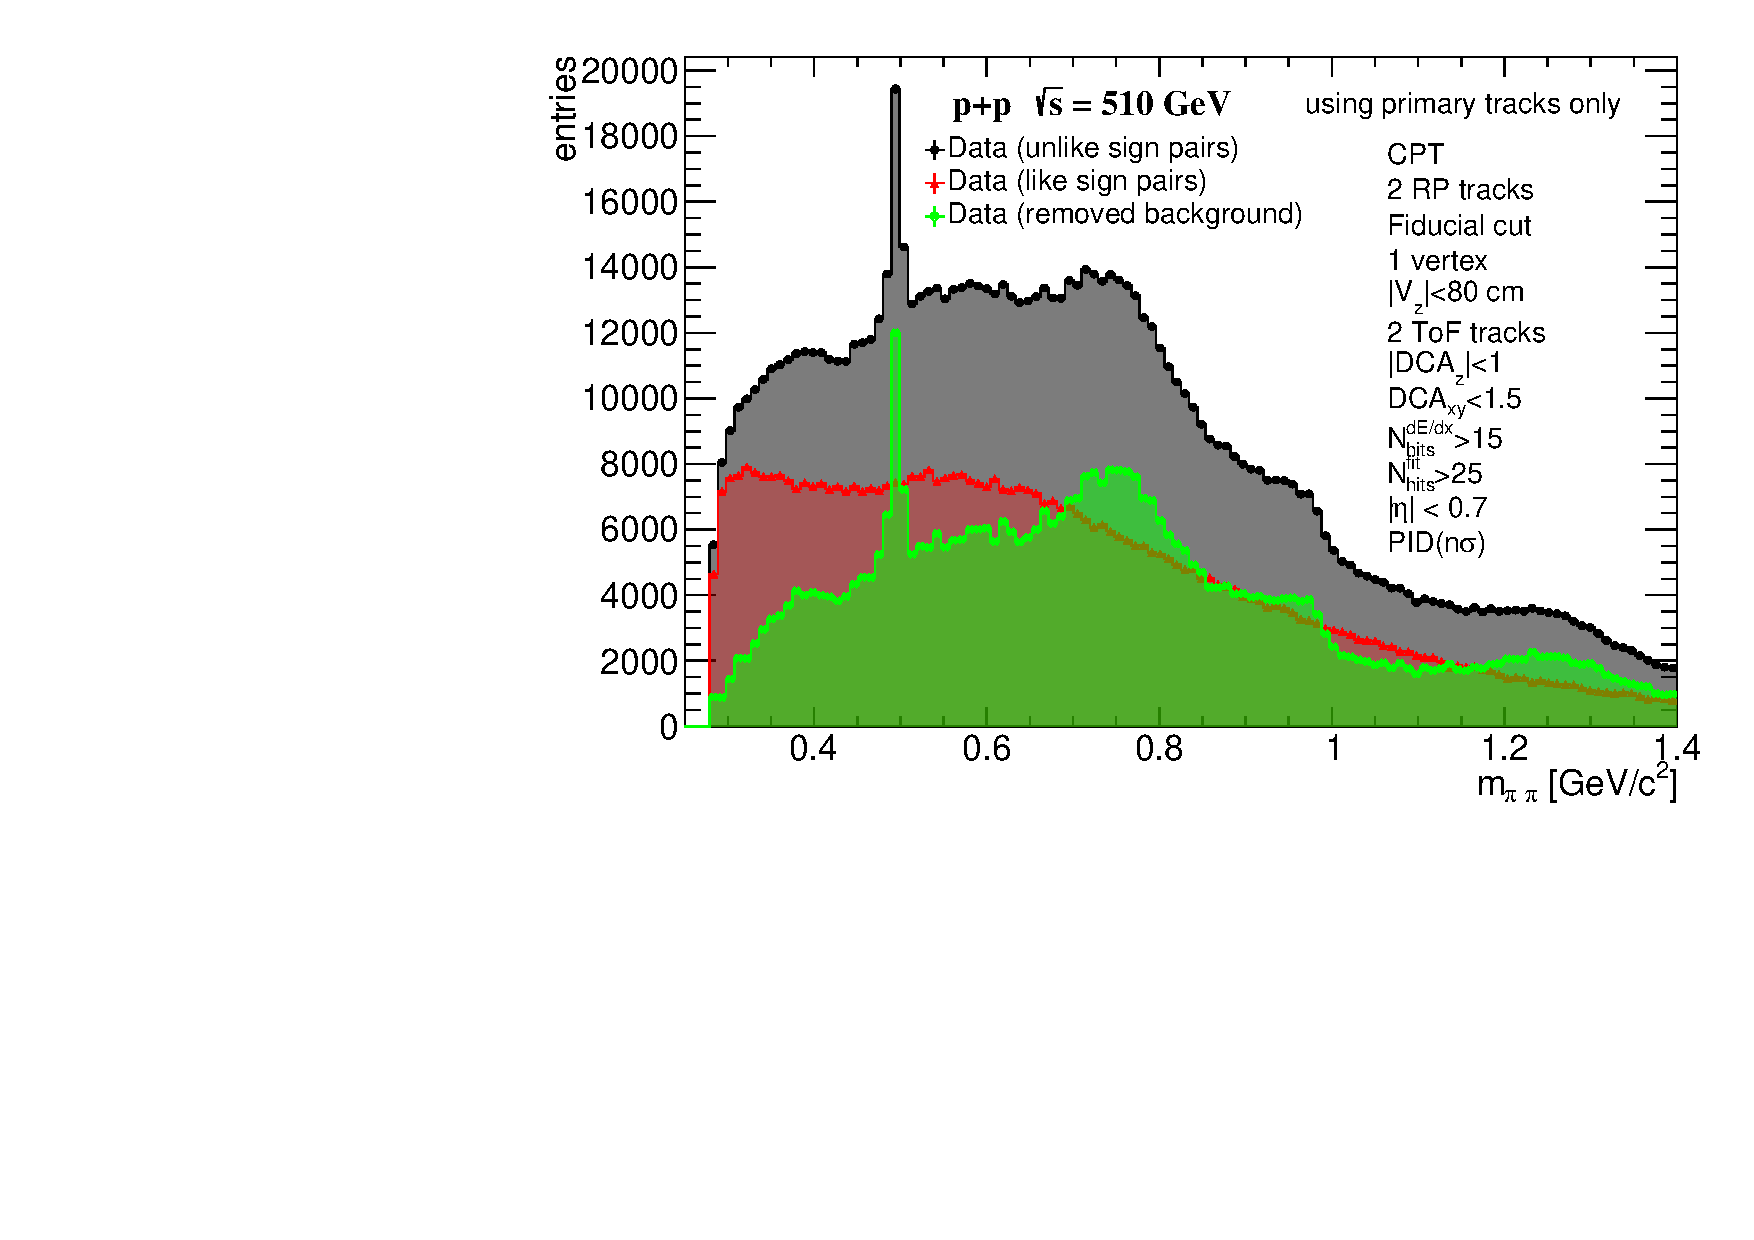
\includegraphics[width=1\textwidth]{figures/invMassLikeUnlikeK0s.pdf}
    \caption[Distribution of invariant mass of $\pi^+ \pi^-$ pairs]{Distribution of invariant mass of identified $\pi^+ \pi^-$ pairs. Black represent the unlike-sign pairs, red the like-sign pairs and green the difference.}
    \label{af10}
\end{figure}
\FloatBarrier
The peak for $K^0_S$ in like-sign pairs was first fitted with Gauss distribution and 1. degree polynomial and later with Gauss distribution and 2. degree polynomial. Functions of both fits are shown as \autoref{er1} and \autoref{er2} respectively. Fits can be seen in \autoref{af11} and \autoref{af13}. Green line represents the fit and red is the polynomial which serves as background. Parameters for red polynomial are the same as for the green fit. 
\newline
\begin{equation}
\centering
f_1(x) = p_0x + p_1x + Ae^{-\frac{(x-\mu)^2}{2\sigma^2}}
\label{er1}
\end{equation}
\begin{equation}
\centering
f_2(x) = p_0x + p_1x + p_2x^2 + Ae^{-\frac{(x-\mu)^2}{2\sigma^2}}
\label{er2}
\end{equation}
The quality of fit is evaluated using the ratio $\frac{\chi^2}{ndf}$. Value $\chi^2$ is the sum of quadratic deviations of fit from the data points. Value $ndf$ stands for number of degrees of freedom\footnote{Value for $ndf$ is calculated as the difference between the number of fitted data points and number of parameters of the fit.}. A good quality fit should have ratio close to 1. Yield was also calculated using the following equation,
\begin{equation}
\centering
y = \frac{1}{norm}(\int^{b}_{a}f_g(x)\mathrm{d}x - \int^{b}_{a}f_r(x)\mathrm{d}x)
\label{er6}
\end{equation}
where $norm$ is a normalization factor and is the size of 1 bin in GeV. Upper and lower  limits of integrals, $a$ and $b$, use values from fit and can be computated as $b=\mu + 3\sigma$ and $a=\mu - 3\sigma$. Results of fit 1 and fit 2, qualities of fits and yields are in \autoref{at1}. 
\FloatBarrier
\begin{figure}[ht]
    \centering
    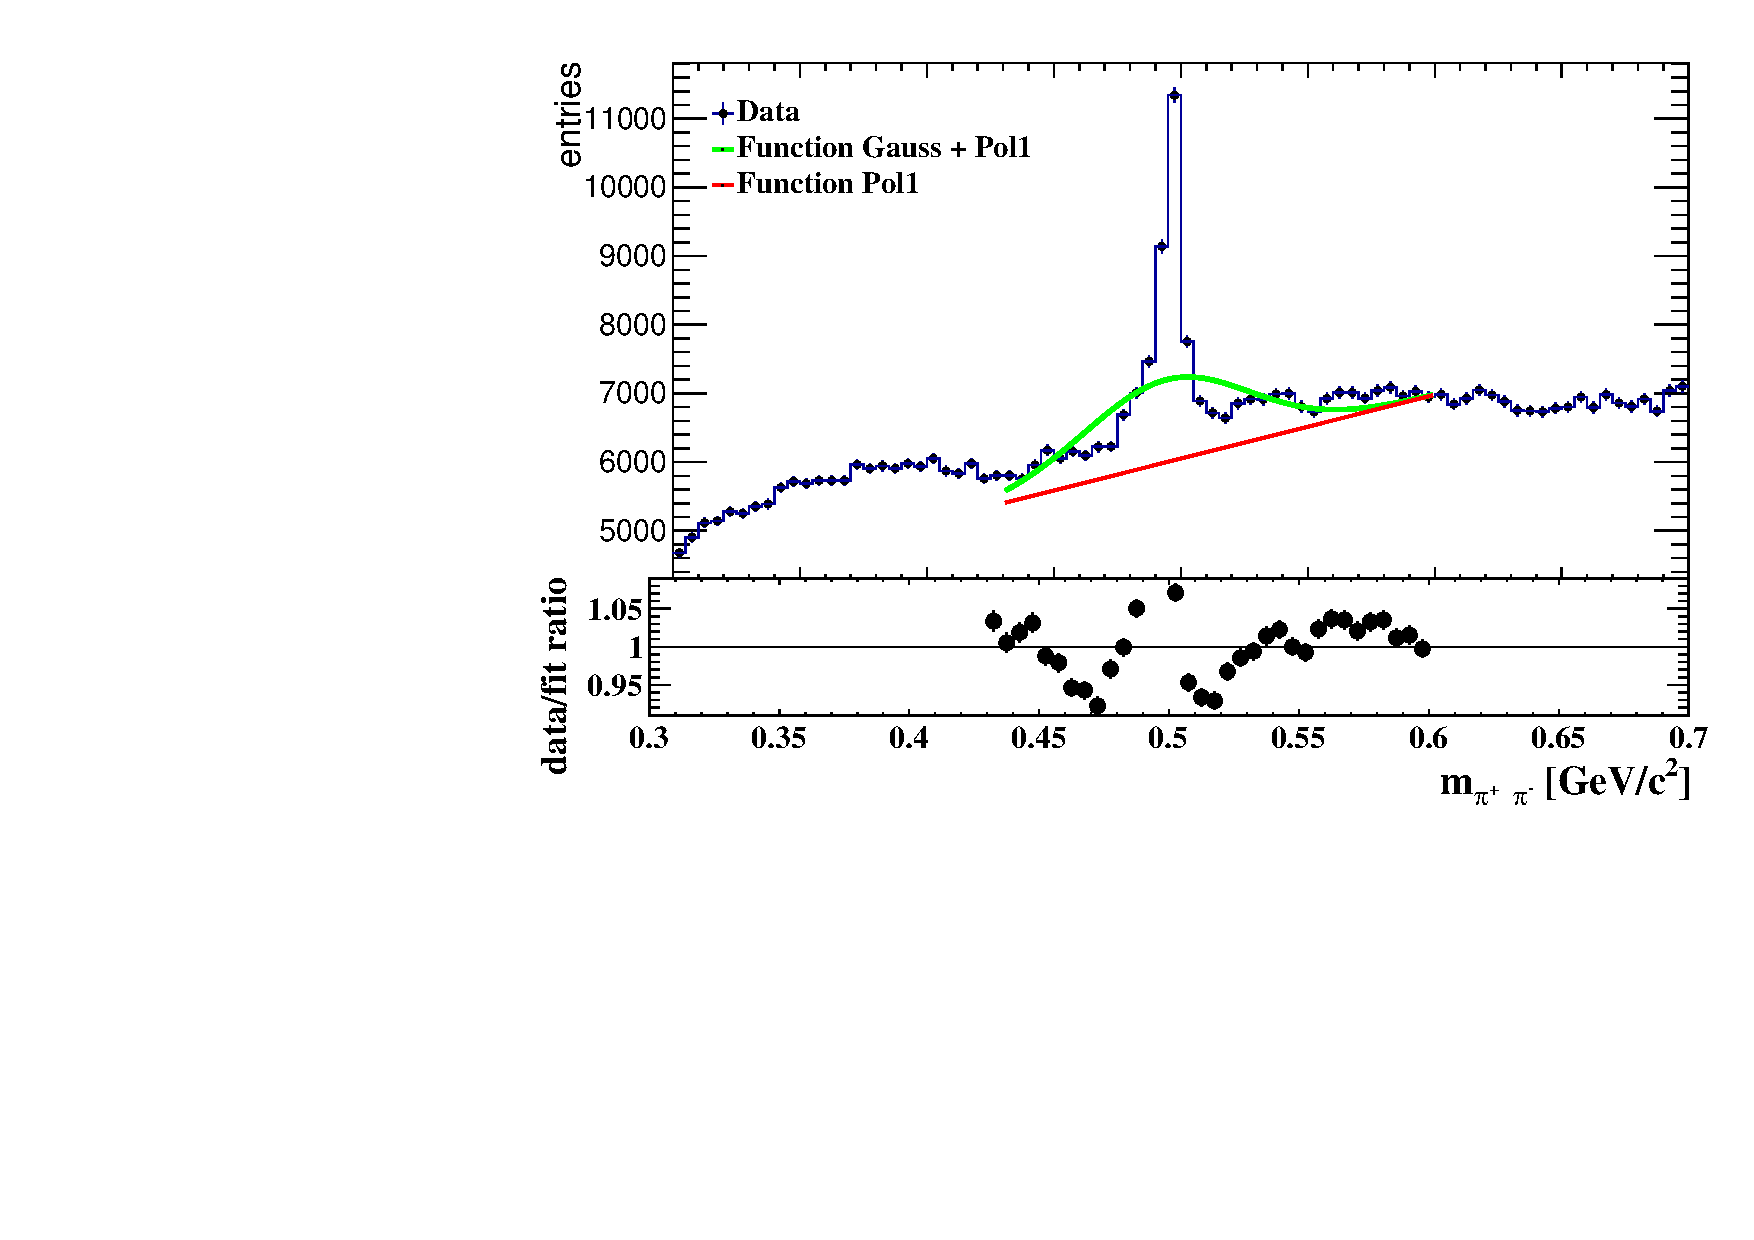
\includegraphics[width=1\textwidth]{figures/K0sFitLinear.pdf}
    \caption[Distribution of invariant pion pairs fitted with Gauss distribution and 1. degree polynomial]{Distribution of invariant mass of $\pi^+ \pi^-$ pairs fitted with a a Gauss distribution function and a first degree polynomial \autoref{er1}. Results of fit are in \autoref{at1}.}
    \label{af11}
\end{figure}
\FloatBarrier

\FloatBarrier
\begin{table}[ht]
    \centering
        \begin{tabular}{c|c|c}
             & Fit 1 & Fit 2 \\ \hline
           $p_0$ & $4.6 \pm 0.2$(stat) $10^{3}$ & $-2.1 \pm 0.3$(stat) $10^{4}$ \\ \hline
           $p_1$ & $1.15 \pm 0.04$(stat) $10^4$ & $1.1 \pm 0.1$(stat) $10^5$\\ \hline
           $p_2$ & & $-1 \pm 1$(stat) $10^4$ \\ \hline
           $A$ & $6.8 \pm 0.1$(stat) $10^3$ &  $6.6 \pm 0.1$(stat) $10^3$ \\ \hline
           $\mu$ & $0.4956 \pm 0.0001$(stat) &  $0.4955 \pm 0.0001$(stat) \\ \hline
           $\sigma$ & $4.79 \pm 0.09$(stat) $10^{-3}$ &  $4.6 \pm 0.1$(stat) $10^{-3}$ \\ \hline
           $a$ & $0.4812$ & $0.4819$\\ \hline
           $b$ & $0.5010$ & $0.5092$ \\ \hline
           $norm$ & $0.008$ & $0.008$ \\ \hline
           $\chi^2$ & $145$ & $57$ \\ \hline
           $ndf$ & $17$  & $16$ \\ \hline
           $\frac{\chi^2}{ndf}$ & $8.5$ & $3.6$  \\ \hline
           $y$ & $10~200 \pm 500$(stat) & $9~400 \pm 300$(stat)
        \end{tabular}
    \caption[Results for fit 1 and 2 of invariant mass of $\pi^+ \pi^-$ pairs]{Results for fit 1 and 2 of peak for $\pi^+ \pi^-$ invariant mass distribution, qualities of fit and yields. Description of variables and the fit functions are in text.}
    \label{at1}
\end{table}
\FloatBarrier
\FloatBarrier
\begin{figure}[ht]
    \centering
        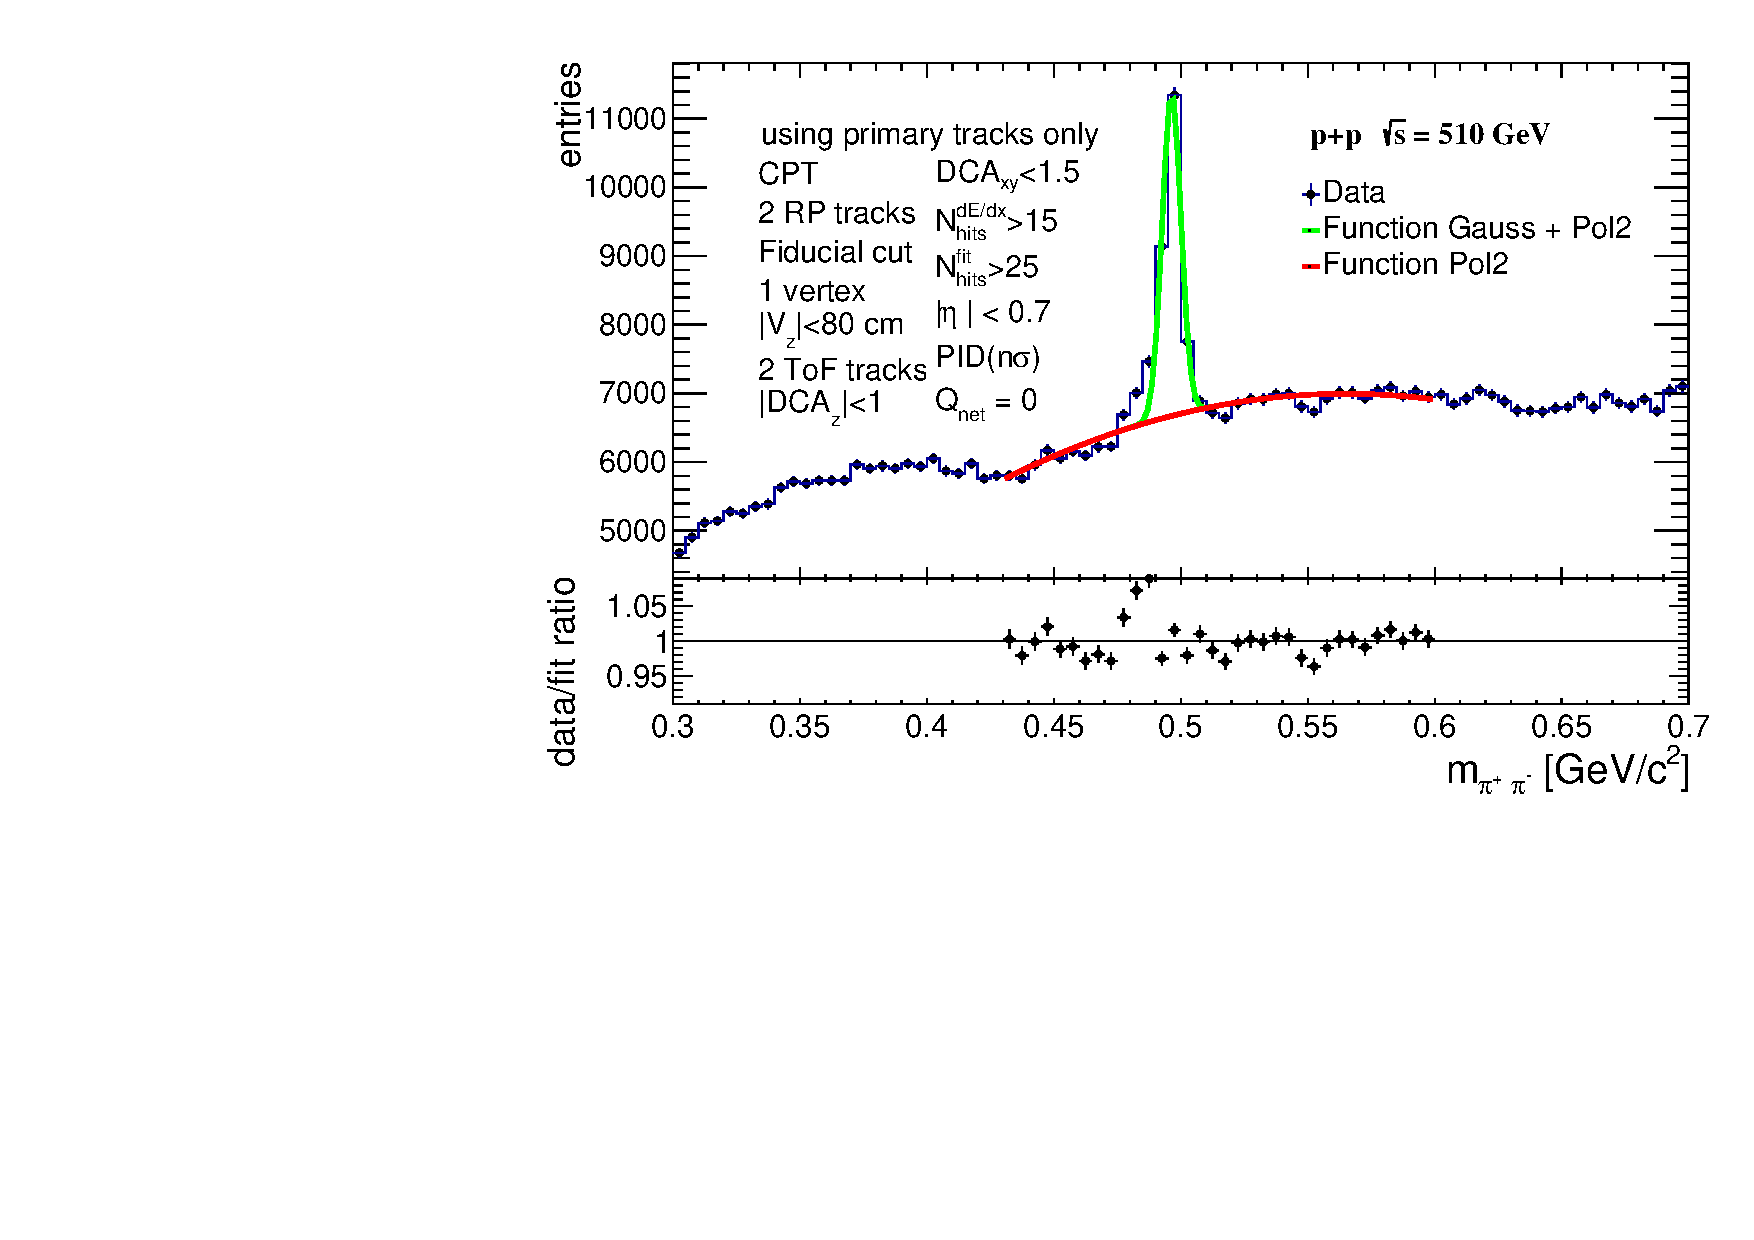
\includegraphics[width=1\textwidth]{figures/K0sFitQuad.pdf}
        \caption[Distribution of invariant pion pairs fitted with Gauss distribution and 2. degree polynomial]{Distribution of invariant mass of $\pi^+ \pi^-$ pairs. Fitted with function of Gauss distribution and second degree polynomial.}
    \label{af13}
\end{figure}
\FloatBarrier
%\FloatBarrier
%\begin{table}[ht]
    %\centering
        %\begin{tabular}{c|c}
           %$p_0$ & $-2.1 \pm 0.3$(stat) $10^{4}$\\ \hline
           %$p_1$ & $1.1 \pm 0.1$(stat) $10^5$ \\ \hline
           %$p_2$ & $-1 \pm 1$(stat) $10^4$ \\ \hline
           %$A$ & $6.6 \pm 0.1$(stat) $10^3$ \\ \hline
           %$\mu$ & $0.4955 \pm 0.0001$(stat) \\ \hline
           %$\sigma$ & $4.6 \pm 0.1$(stat) $10^{-3}$ \\ \hline
           %$a$ & $0.4819$ \\ \hline
           %$b$ & $0.5092$ \\ \hline
           %$norm$ & $0.008$ \\ \hline
           %$\chi^2$ & $57$ \\ \hline
           %$ndf$ & $16$  \\ \hline
           %$\frac{\chi^2}{ndf}$ & $3.6$ \\ \hline
           %$y$ & $9~400 \pm 300$(stat)
        %\end{tabular}
    %\caption[Results for fit 2 of invariant mass of $\pi^+ \pi^-$ pairs]{Results of fitted peak for $\pi^+ %\pi^-$ invariant mass distribution, quality of fit and yield. Fit function is shown in \autoref{er2}.}
    %\label{at2}
%\end{table}
%\FloatBarrier
The expected value, $\mu$, which was fitted as parameter in both fits, represents the decay channel of $K^0_S$ and it's invariant mass. Values from both fits correspond to official PDG value of invariant mass of $K^0$: $497.611$  $\pm$ 0.013 MeV. 
\newline
To take a closer look at exclusive production of $K^0_S$, the missing transverse momentum was computed\footnote{Momenta of 4 measured particles (2 forward protons and 2 central pions) in $(x,y)$ directions were summed.}. Exclusive production would mean the missing transverse momentum would within 0. Distribution of missing transverse momentum is shown in \autoref{af49} with a cut at 100 MeV. The distribution of invariant mass of candidates that passed this condition is shown in \autoref{af50}.

\FloatBarrier
\begin{figure}[ht]
    \centering
    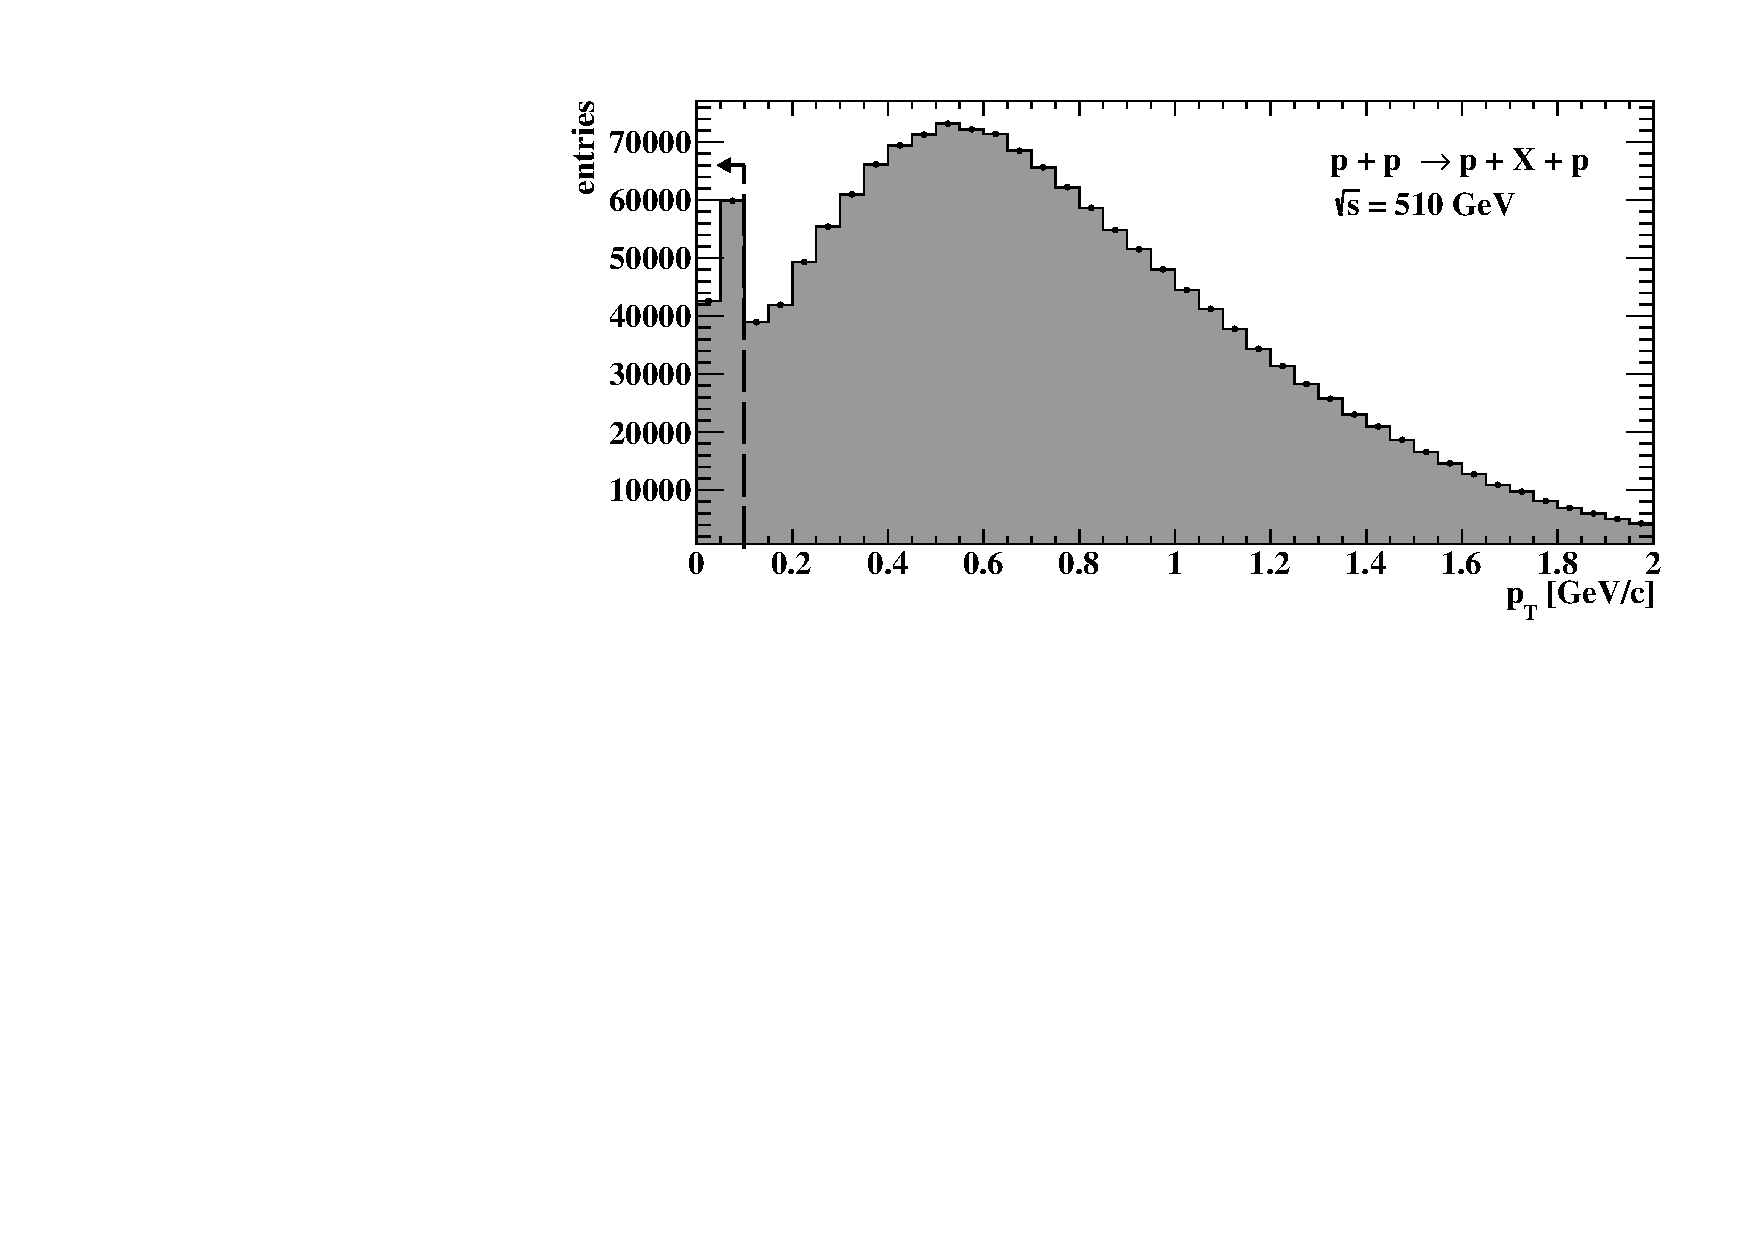
\includegraphics[width=1\textwidth]{figures/hPtMissingK0s.pdf}
    \caption[Distribution of missing transverse momentum for $\pi \pi$ pairs]{Distribution of missing transverse momentum for particle $\pi^+ \pi^-$ pairs. Arrow represents a cut at 100 MeV.}
    \label{af49}
\end{figure}
\FloatBarrier

\FloatBarrier
\begin{figure}[ht]
    \centering
    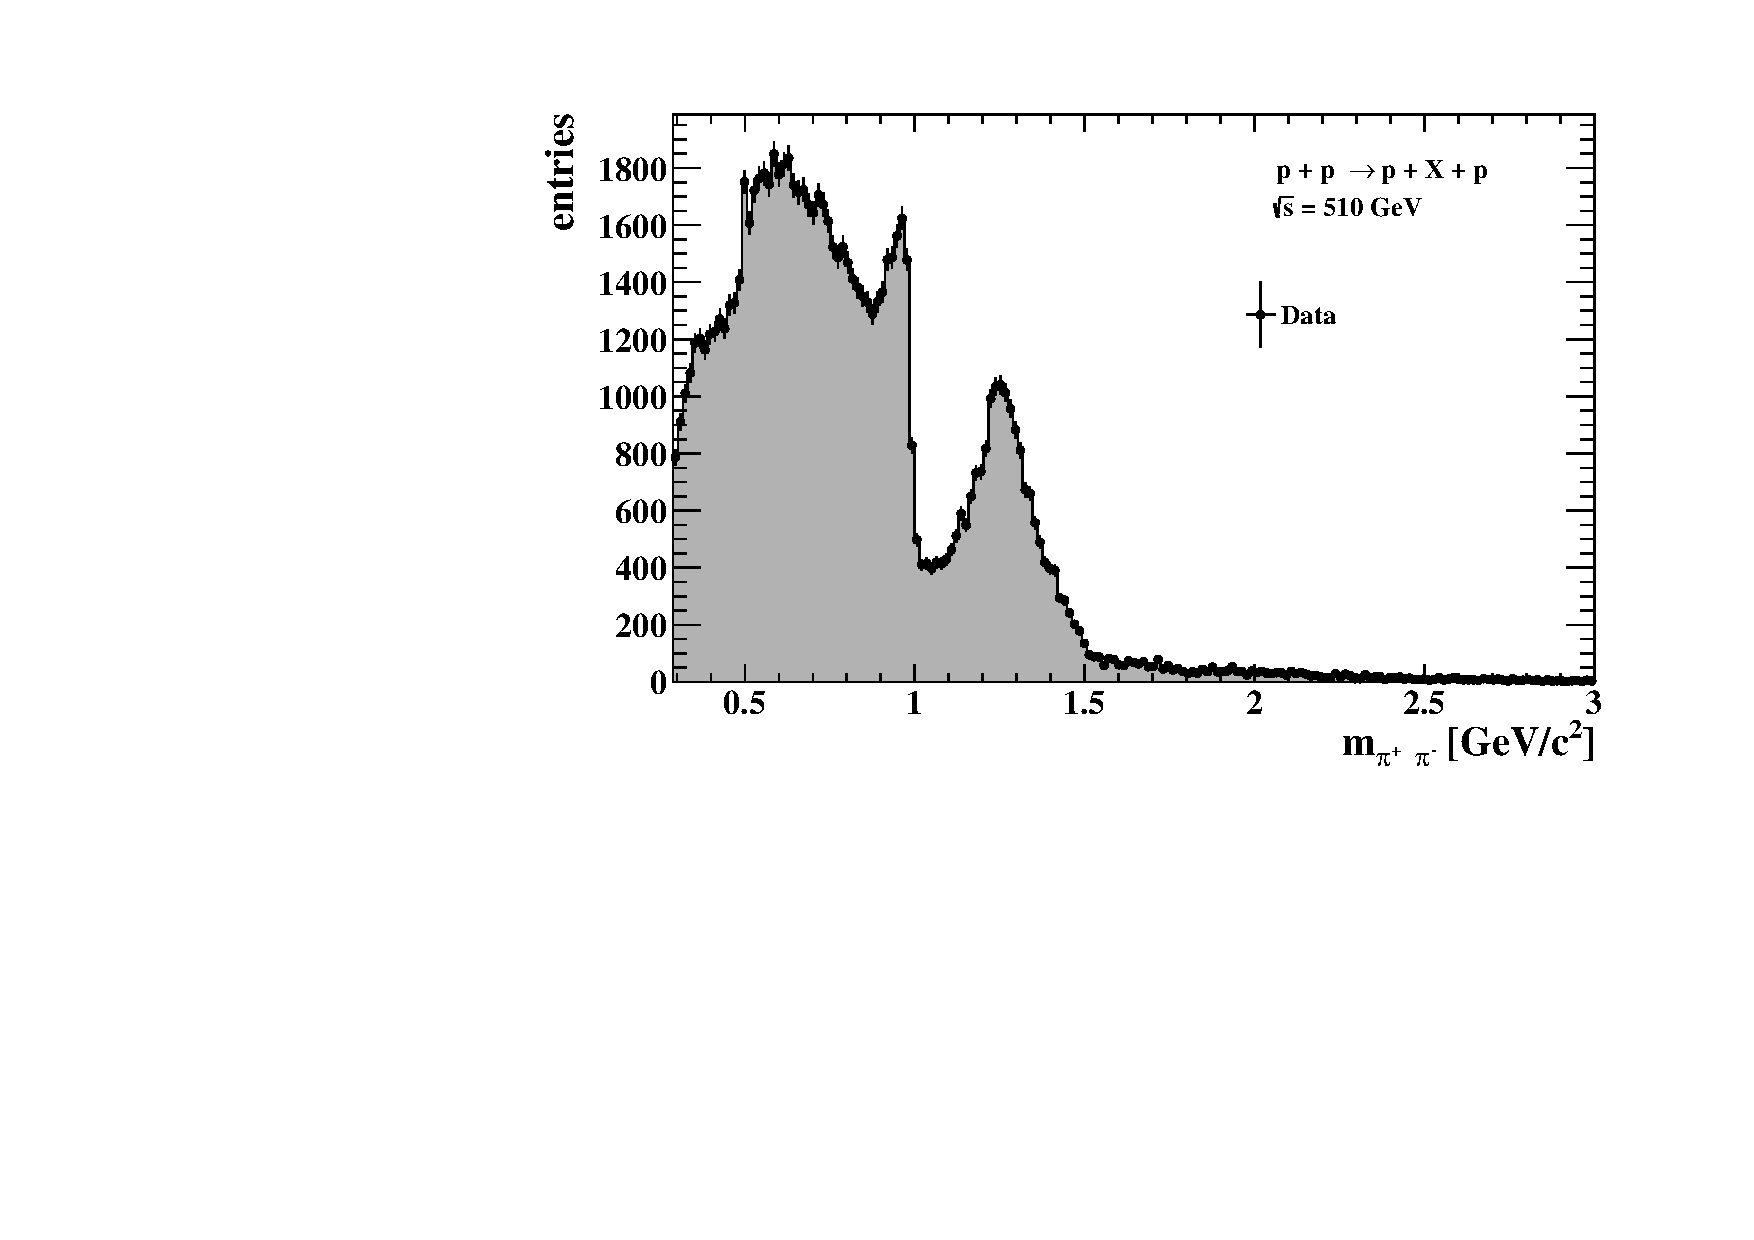
\includegraphics[width=1\textwidth]{figures/invMassPiPiexclusive.pdf}
    \caption[Distribution of invariant mass of exclusively produced $\pi \pi$ pairs]{Distribution of invariant mass of $\pi \pi$ pairs that were created with exclusive production. Black points represent unlike-sign pairs and red like-sign.}
    \label{af50}
\end{figure}
\FloatBarrier

Distribution shown in \autoref{af50} has many similarities to distributions discussed in \autoref{theoretics}, \autoref{recent}. They were visible even without the condition for exclusive production in \autoref{af10}, but the structures here are much more significant. Even though it is within the uncertainties, a slight peak at around 500 MeV can be seen which could represent $K^0_S$. If it was more significant, it could mean some level of contamination of data. Distribution then rises and later decreases. Sharp peak right before 1 GeV which corresponds to resonance $f_0$(980) followed by a very steep drop. Resonance $f_2$(1270) at 1270 MeV can also be seen as a tall and wide peak. All of these correspond to results discussed in \autoref{theoretics}, \autoref{recent}. 

\section{Results for $\Lambda^0$}
\label{Lambda}
Particle $\Lambda^0$ and it's antiparticle $\overline{\Lambda}^0$ are neutral baryons\footnote{Baryons are particles composed out of 3 quarks.} which mostly decay to $p \pi^-$ and $\overline{p} \pi^+$ respectively\footnote{Decay $\Lambda^0 \longrightarrow \overline{p} \pi^+$ is forbidden because it does not satisfy the law of conservation of baryon number.}. Second most probable decay for $\Lambda^0$ is into pair $\pi^0 n$.


\FloatBarrier
\begin{figure}[ht]
    \centering
    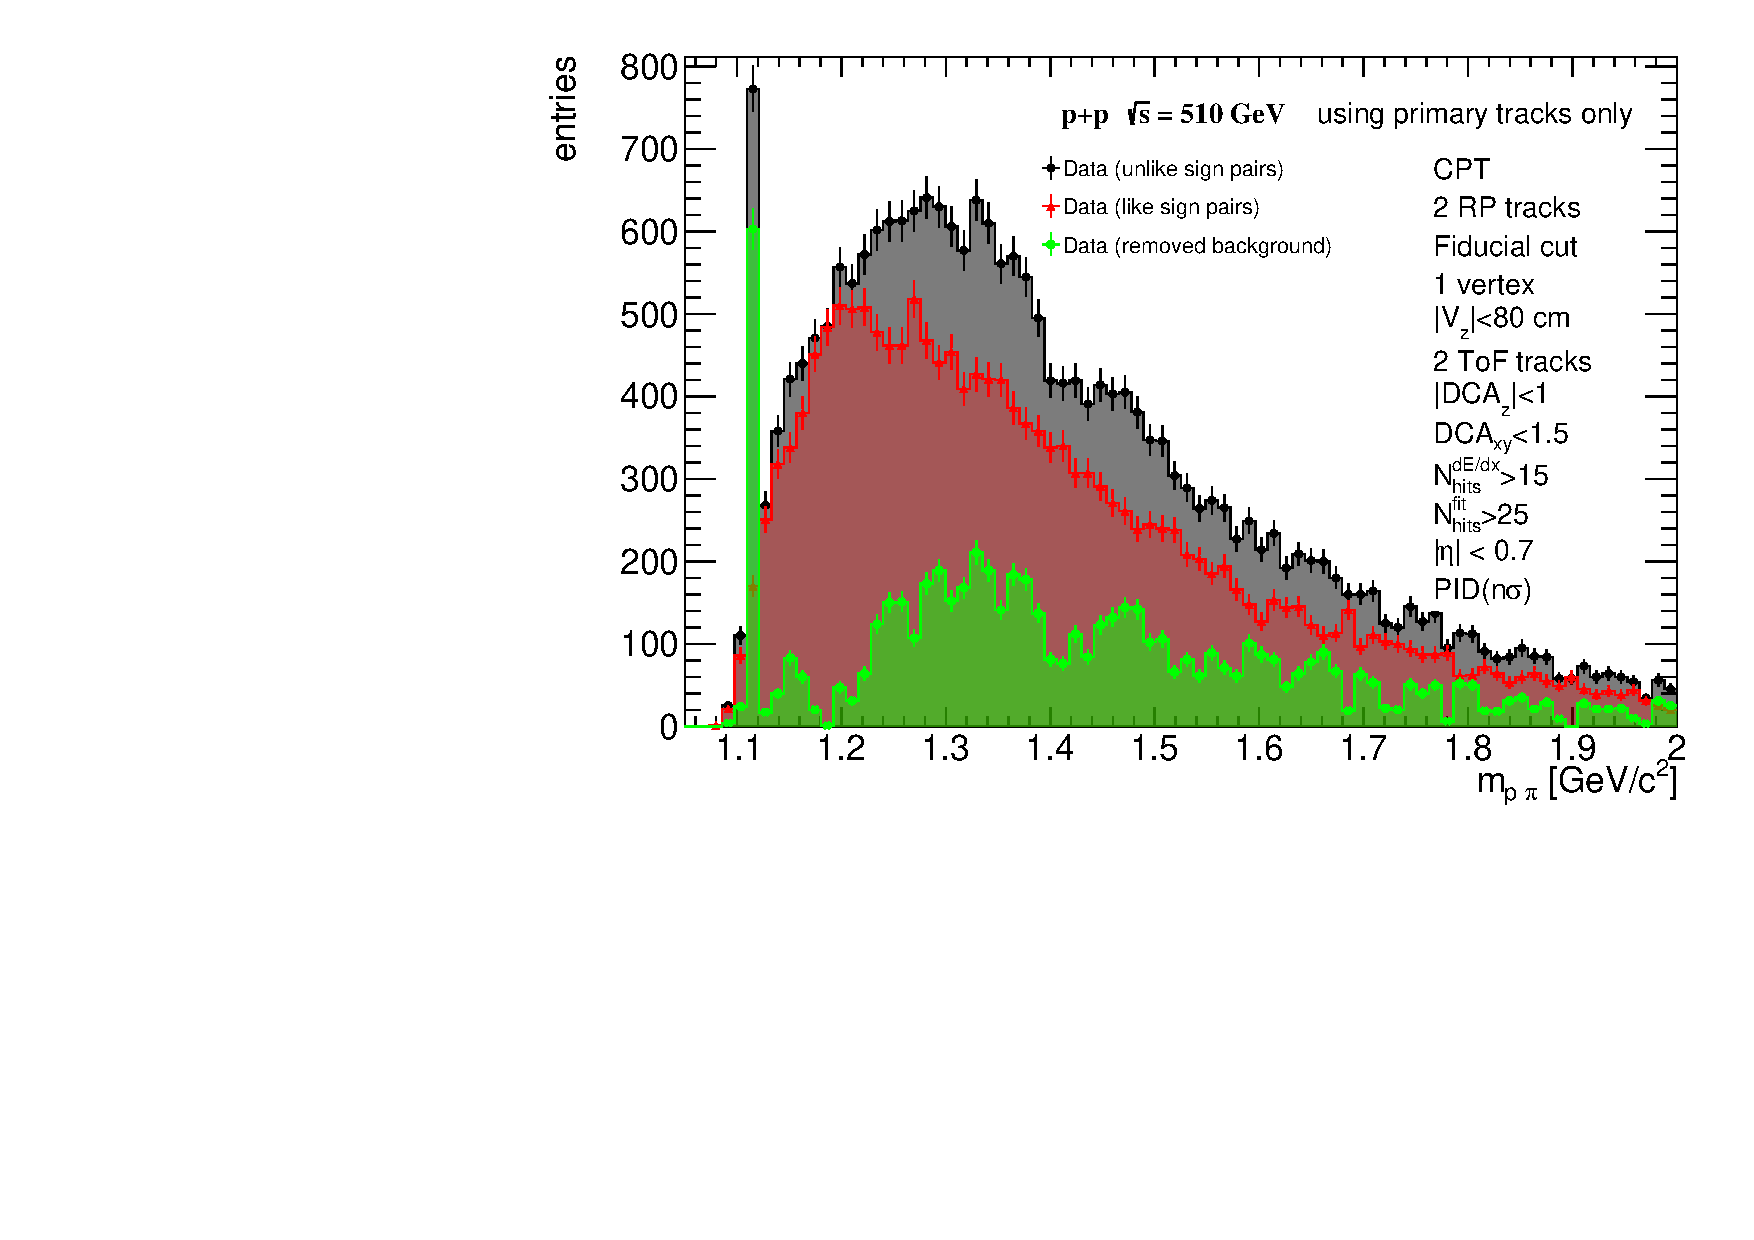
\includegraphics[width=1\textwidth]{figures/invMassLikeUnlikeLambda.pdf}
    \caption[Results for fit 1 of invariant mass of $p \pi$ pairs]{The distribution of invariant mass for identified $p \pi$ pairs.  Black represent the unlike-sign pairs, red the like-sign pairs and green the difference.}
    \label{af14}
\end{figure}
\FloatBarrier
Invariant mass distributions of $p \pi$ pairs are shown in \autoref{af14}. Black represents unlike-sign pairs, red like-sign pairs and green is the difference. Peak at around $1.1$ GeV is the $\Lambda^0$ or $\overline{\Lambda}^0$. The statistics for this distribution is much smaller than for $K^0_S$ and the background is of similar scale to unlike-sign pairs. Therefore, the green signal, aside from $\Lambda$ peak, is quite small. Only possible structure is a slight dip at around $1.4$ GeV. Otherwise, like- and unlike-sign pair distributions have very similar shapes. 
\FloatBarrier
\begin{figure}[ht]
    \centering
    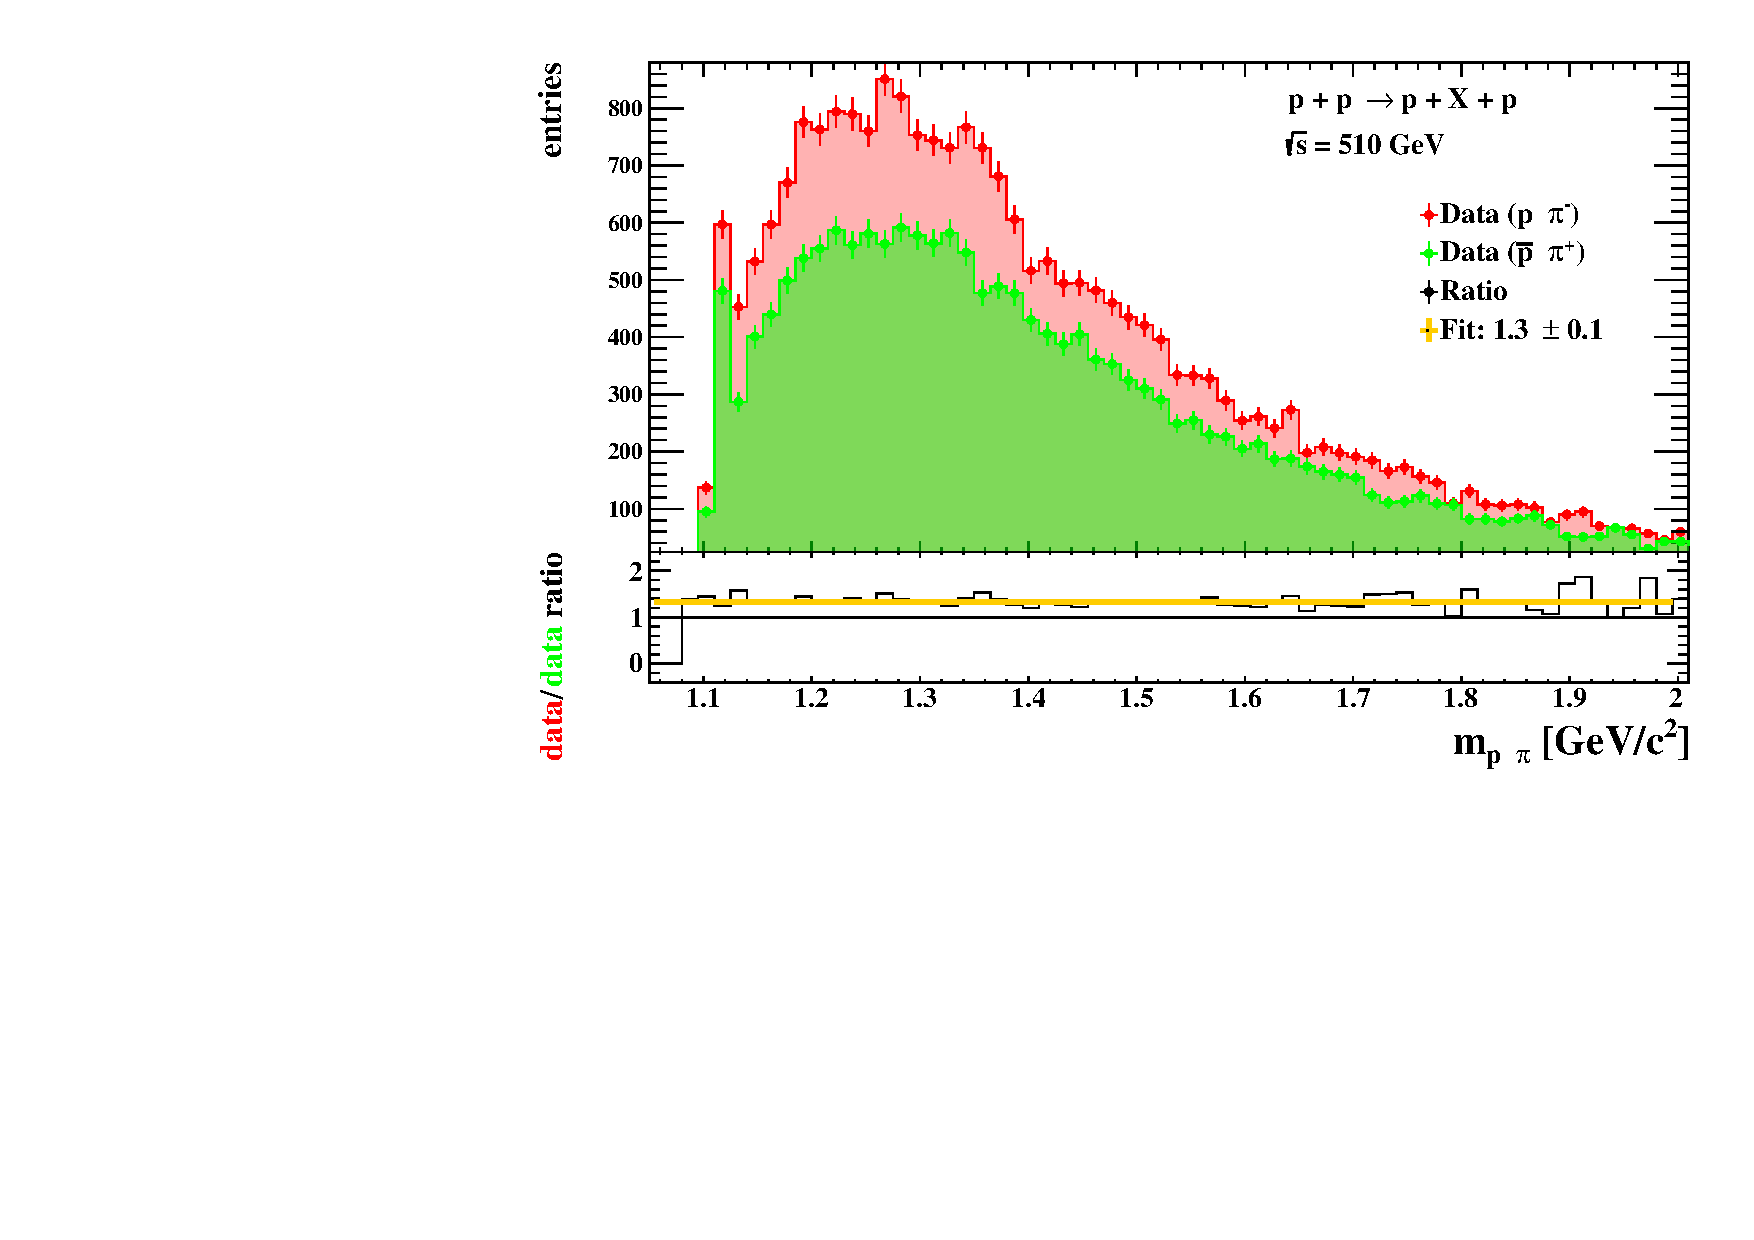
\includegraphics[width=1\textwidth]{figures/LambdaAntiLambda.pdf}
    \caption[Distributions of invariant mass for $p \pi^-$ and $\overline{p} \pi^+$ pairs]{Distributions of invariant mass for $p \pi^-$ (green) and $\overline{p} \pi^+$ (red) pairs. Underneath is a ratio plot which is fitted with a constant function.}
    \label{af19}
\end{figure}
\FloatBarrier

\FloatBarrier
\begin{figure}[ht]
    \centering
    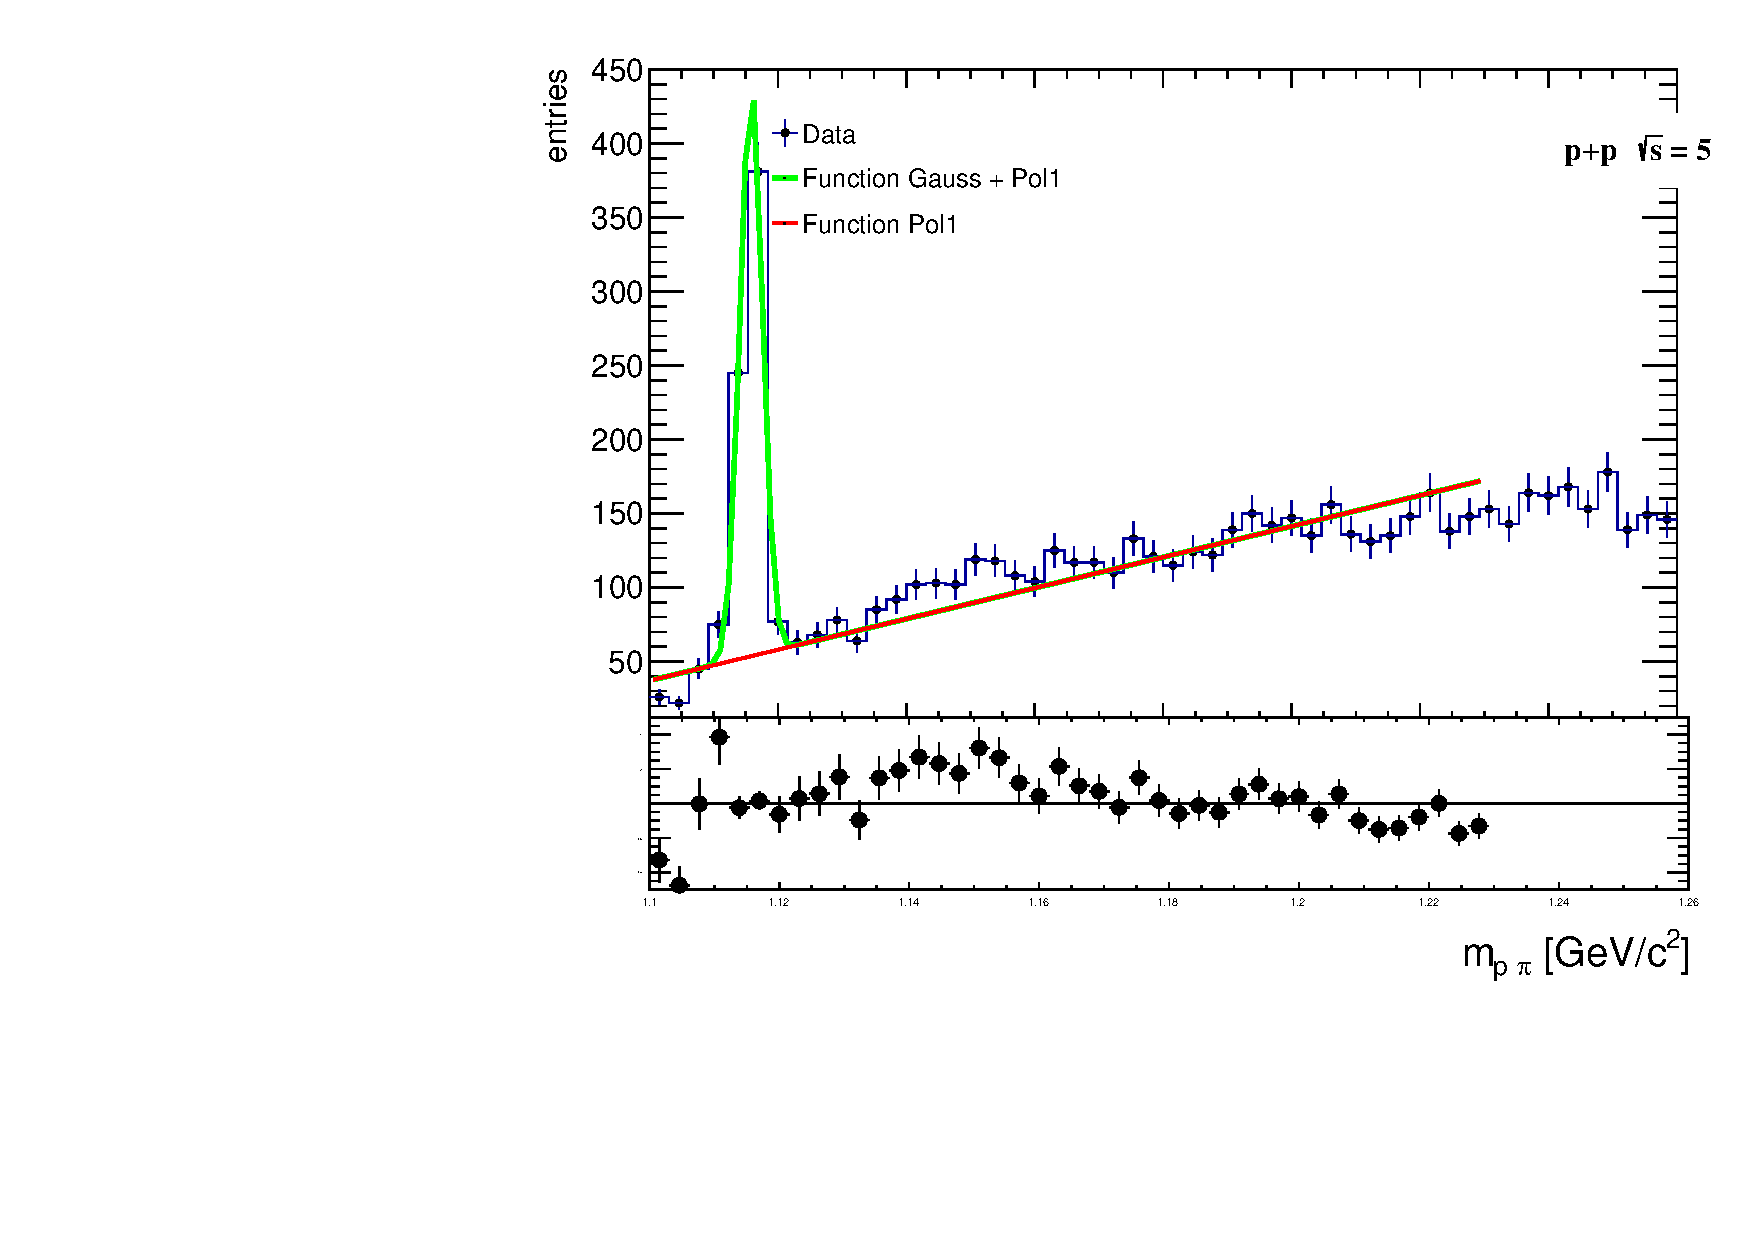
\includegraphics[width=1\textwidth]{figures/LambdaFitLinear.pdf}
    \caption[Distribution of invariant pion proton pairs fitted with Gauss distribution and 1. degree polynomial]{The distribution of invariant mass for identified $p$ $\pi$ pairs fitted with Gauss distribution function and first degree polynomial. Results of fit can be found in \autoref{at3}.}
    \label{af15}
\end{figure}
\FloatBarrier
\autoref{af19} shows the difference between $p \pi^-$ and $\overline{p} \pi^+$ distributions. Shapes of the distributions are very similar- both follow the distributions shown in \autoref{af14} which is the expected shape. The only noticeable difference is the scaling of both structures. Ratio of measured data is underneath and is fitted with a constant function. The result of fit: $1.3 \pm 0.1$. This could possibly be because of lower efficiency in measuring antimatter.
\newline
Peaks from unlike-sign distributions of invariant mass for $p \pi$ pairs were fitted similarly to fits for $K^0_S$. First fit was Gauss distribution and 1. degree polynomial shown in \autoref{er1}. Second fit was again, Gauss distribution and 2. degree polynomial and can be found in \autoref{af16}. Results of both fits can be found in \autoref{at3}. The qualities of fits were calculated the same way as for $K^0_S$. 
\FloatBarrier
\begin{table}[ht]
        \centering
        \begin{tabular}{c|c|c}
             & Fit 1 & Fit 2 \\ \hline
           $p_0$ & $-1.02 \pm 0.04$(stat) $10^{3}$ & $-1.105$ $ \pm$ $ 0.0002$(stat) $10^{4}$ \\ \hline
           $p_1$ & $9.6 \pm 0.04$(stat) $10^2$ &  $1.829$ $ \pm$ $ 0.0002$(stat) $10^4$  \\ \hline
           $p_2$ & $-7.48$ $ \pm$ $ 0.01$(stat) $10^3$ \\ \hline
           $A$ & $3.6 \pm 0.2$(stat) $10^2$ & $3.6$ $ \pm$ $ 0.2$(stat) $10^3$ \\ \hline
           $\mu$ & $1.11569$ $ \pm$ $ 0.00009$(stat) & $1.11567$ $\pm$ $ 0.00007$(stat)  \\ \hline
           $\sigma$ & $1.70$ $ \pm$ $ 0.07$(stat) $10^{-3}$ &  $1.71$ $ \pm$ $ 0.07$(stat) $10^{-3}$\\ \hline
           $a$ & $1.1106$ & $1.1105$\\ \hline
           $b$ & $1.1208$ &$1.1208$ \\ \hline
           $\chi^2$ & $94$ & $41$\\ \hline
           $ndf$ & $41$  &  $37$\\ \hline
           $\frac{\chi^2}{ndf}$ & $2.3$ & $1.1$ \\ \hline
           $y$ & $540 \pm 50$(stat) & $540 \pm 50$(stat)
        \end{tabular}
    \caption[Results for fit 1 and 2 of invariant mass of $p \pi$ pairs.]{Results of fits for peak of $p ~\pi^- $ and $\overline{p}~\pi^+$ invariant mass distribution, quality of fit and yield. Description of variables is in text. }
    \label{at3}
\end{table}
\FloatBarrier
Gauss distribution follows the peak in both fits very well. The quality test $\frac{\chi^2}{ndf}$ of both fits is better compared to $K^0_S$ fits. Especially the second fit for $\Lambda$. When it comes to modeling the shape of the background, 2. degree polynomial is superior to 1. degree polynomial. The expected values for both fits, $\mu$, correspond to PDG value for invariant mass of particle $\Lambda^0$: $1115.683$ $\pm$ $0.006$ MeV \cite{zyla}.
\newline
Missing transverse momentum for $p \pi$ pairs is drawn in \autoref{af77}. The shape of the distribution is as expected. Exclusive production for $\Lambda$ is forbidden because it does not satisfy the law of conservation of strangeness.
\FloatBarrier
\begin{figure}[ht]
    \centering
    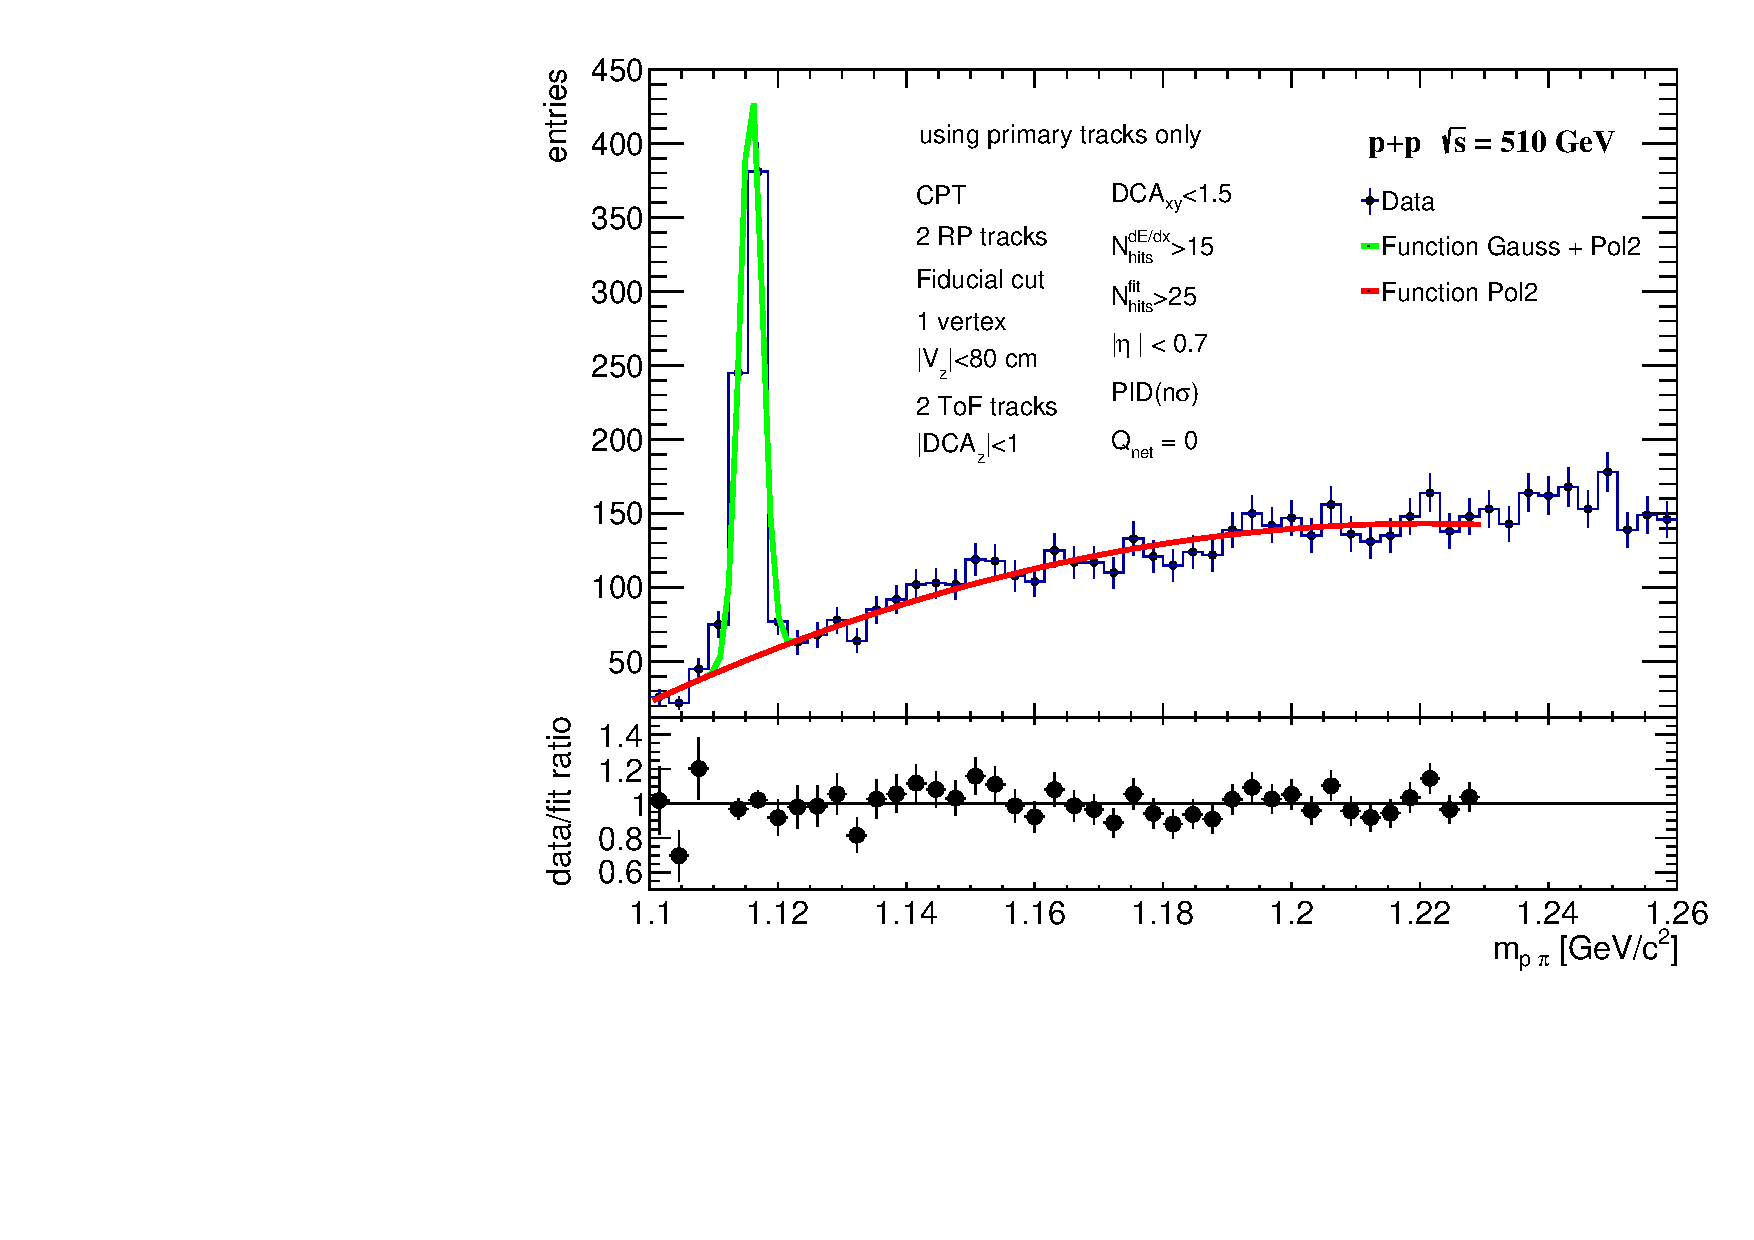
\includegraphics[width=1\textwidth]{figures/LambdaFitQuad.pdf}
    \caption[Distribution of invariant pion proton pairs fitted with Gauss distribution and 2. degree polynomial.]{The distribution of invariant mass of identified $p$ $\pi$ pairs fitted with Gauss distribution function and second degree polynomial.}
    \label{af16}
\end{figure}
\FloatBarrier

%\FloatBarrier
%\begin{table}[ht]
   %    \centering
%        \begin{tabular}{c|c}
%           $p_0$ & $-1.105$ $ \pm$ $ 0.0002$(stat) $10^{4}$\\ \hline
%           $p_1$ & $1.829$ $ \pm$ $ 0.0002$(stat) $10^4$ \\ \hline
%           $p_2$ & $-7.48$ $ \pm$ $ 0.01$(stat) $10^3$ \\ \hline
%           $A$ & $3.6$ $ \pm$ $ 0.2$(stat) $10^3$ \\ \hline
%           $\mu$ & $1.11567$ $\pm$ $ 0.00007$(stat) \\ \hline
%           $\sigma$ & $1.71$ $ \pm$ $ 0.07$(stat) $10^{-3}$ \\ \hline
%           $a$ & $1.1105$ \\ \hline
%           $b$ & $1.1208$ \\ \hline
%           $\chi^2$ & $41$ \\ \hline
%           $ndf$ & $37$  \\ \hline
%           $\frac{\chi^2}{ndf}$ & $1.1$ \\ \hline
%           $y$ & $540 \pm 50$(stat)
%        \end{tabular}
%    \caption[Results for fit 2 of invariant mass of $p \pi$ pairs]{Results of fitted peak for $p$ $\pi^- $ and $\overline{p}$ $\pi^+$ invariant mass distribution, quality of fit and yield. Fitted with Gauss distribution and 2. degree polynomial.}
%    \label{at4}
%\end{table}
%\FloatBarrier

\FloatBarrier
\begin{figure}[ht]
    \centering
    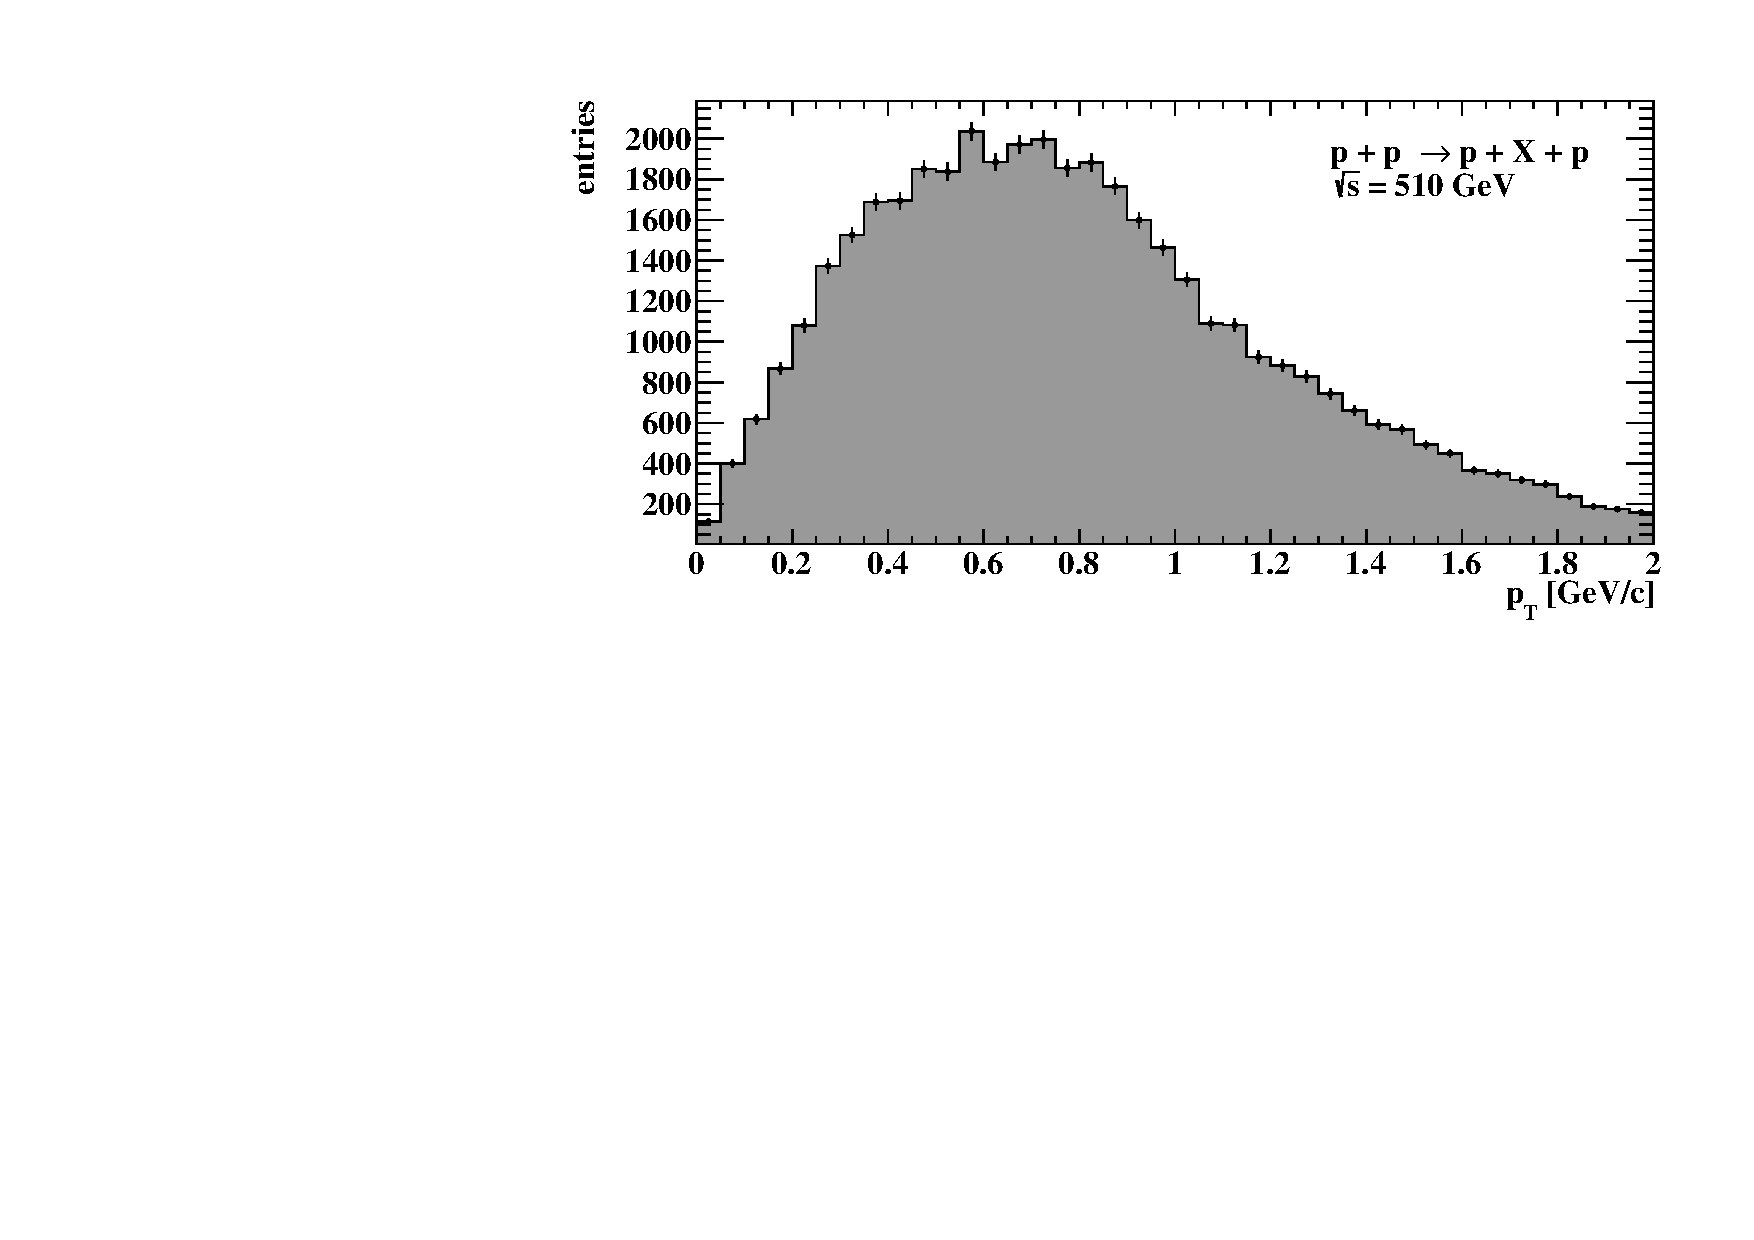
\includegraphics[width=1\textwidth]{figures/hPtMissingLambda.pdf}
    \caption[Distribution of transverse momenta for $p \pi$ pairs]{Distribution of transverse momenta for $p \pi$ pairs.}
    \label{af77}
\end{figure}
\FloatBarrier
